\documentclass{article}
\author{Richard Gendal Brown, James Carlyle, Ian Grigg, Mike Hearn}
\date{August, 2016}
\title{Corda: Introducción}
%%\setlength{\parskip}{\baselineskip}
\usepackage{amsfonts}
\usepackage{listings}
\usepackage{color}
\usepackage{epigraph}
\usepackage{graphicx}
\graphicspath{ {images/} }
\usepackage[export]{adjustbox}
\usepackage{float}
\usepackage{hyperref}
\usepackage[super,comma,sort&compress]{natbib}
\usepackage[nottoc]{tocbibind}
%\usepackage[natbibapa]{apacite} 
\renewcommand{\thefootnote}{\alph{footnote}}

%\epigraphfontsize{\small\itshape}
\setlength\epigraphwidth{4.5cm}
\setlength\epigraphrule{0pt}

\begin{document}

\maketitle 

\begin{abstract}
Un registro contable distribuido constituido por nodos sin relación de confianza permitiría la existencia de una única base de datos global que registre el estado de acuerdos y obligaciones entre instituciones y personas. Esto eliminaría gran parte del dilatado esfuerzo manual requerido actualmente para mantener sincronizados entre sí registros contables dispares. Permitiría también mayores niveles de compartición de código que los utilizados actualmente en el sector financiero, reduciendo para todos el coste de los servicios financieros. Presentamos Corda, una plataforma diseñada para alcanzar esos objetivos. Este artículo proporciona una introducción de alto nivel destinada al público en general. Un artículo técnico de próxima publicación tratará en mayor detalle el diseño y las decisiones arquitectónicas fundamentales.
\end{abstract}
\newpage
\tableofcontents
\newpage
\section{Introducción}
En R3, creemos que la tecnología de registro contable distribuido tiene el potencial de transformar el sector de los servicios financieros en beneficio tanto de los clientes como de las empresas que participan en el mismo. Contemplamos un futuro en el que los acuerdos financieros queden registrados y gestionados automáticamente, sin errores, en el que todo el mundo pueda llevar a cabo transacciones con cualquier fin contractual, sin contratiempos ni fricciones. Creemos que los mercados van a evolucionar hacia modelos en los que las partes de los acuerdos financieros los registren solamente una vez y colaboren para mantener registros exactos y compartidos de dichos acuerdos. Las duplicaciones, reconciliaciones, coincidencias fallidas e interrupciones serán cosa del pasado. No habrá más áreas aisladas de representación de activos.

Aspiramos a definir un tejido de registros contables compartidos para los escenarios de uso de los servicios financieros que pueda ser implantado en los marcos legales existentes y que se base en tecnologías contrastadas. Nuestra filosofía puede ser desglosada en tres categorías: ingeniería para los requisitos de las instituciones, énfasis en los requisitos no funcionales, y extensibilidad.

Este artículo introduce las características de diseño de la plataforma Corda, que, en nuestra opinión, la convierten en una opción atractiva para las instituciones financieras reguladas.\footnote{Pueden ponerse en contacto con los autores por correo electrónico: Richard Gendal Brown \href{mailto:richard@r3cev.com}{(richard@r3cev.com)}, James Carlyle \href{mailto:james@r3cev.com}{(james@r3cev.com)}, Ian Grigg \href{mailto:iang@r3cev.com}{(iang@r3cev.com)}, Mike Hearn \href{mailto:mike@r3cev.com}{(mike@r3cev.com)}}

\section{Contexto}
Los bancos se cuentan entre los primeros que adoptaron las tecnologías de la información y, pese a la creencia popular, han hecho un buen trabajo automatizando procesos que antes eran manuales y digitalizando procesos que antes eran físicos. Sin embargo, existen oportunidades significativas para la mejora del coste y la eficiencia de las arquitecturas que emergieron en su momento. 

En particular, cada una de las instituciones financieras mantiene sus propios registros contables, que registran la imagen de esa empresa de sus acuerdos y posiciones respecto al conjunto de sus clientes y sus contrapartes. Dichas contrapartes, a su vez, mantienen sus propias imágenes Esta duplicación puede llevar a inconsistencias, y da lugar a la necesidad de una armonización, reconciliación y resolución de errores costosas por y entre las diversas partes de una transacción. En la medida que persisten las diferencias entre la imagen de dos empresas sobre la misma transacción, existe también una fuente de riesgos, algunos de ellos potencialmente sistémicos.

La pluralidad de instituciones financieras genera competencia y posibilidades de elección, pero la pluralidad de plataformas tecnológicas en la que se basa genera complejidad y provoca riesgos operativos. Sin embargo, hasta hace poco esto era inevitable: salvo para infraestructuras de mercado centralizadas\footnote{Ejemplos de ello serían el Depository Trust \& Clearing Corporation (DTCC) y Continuous Linked Settlement Group (CLS).}, había pocas formas eficaces de consolidar la tecnología entre empresas sin que también se consolidaran éstas.

Los servicios de infraestructura de los mercados centralizados han avanzado algo hacia el incremento de la lógica de negocio y cantidad de datos compartidos entre las empresas, pero, en conjunto, el grado de integración conseguido en el mundo de las transacciones financieras sigue estando muy por detrás de lo que se ha conseguido en el mundo del intercambio de información desde el advenimiento de internet. \cite{IT}

Creemos que la madurez de las técnicas criptográficas, ejemplificada en parte por lo que es vulgarmente conocido como «tecnología blockchain» (tecnología de cadena de bloques), proporciona una nueva oportunidad: la posibilidad de sistemas fehacientes de registro compartidos de forma segura entre las empresas. Este enfoque proporciona la oportunidad de transformar la economía de las empresas financieras, en particular, pero no de forma exclusiva, en los servicios post-negociación, implantando una nueva plataforma compartida para registrar los eventos financieros y procesar la lógica de negocio: una en la que un único registro contable lógico global tiene carácter fehaciente para todos los acuerdos entre empresas registrados en el mismo. Esta arquitectura definirá una nueva plataforma compartida para la industria, sobre la cual pueden competir los que ya están establecidos, los recién llegados y los terceros, para proporcionar nuevos e innovadores productos y servicios. 

\begin{figure}[H]
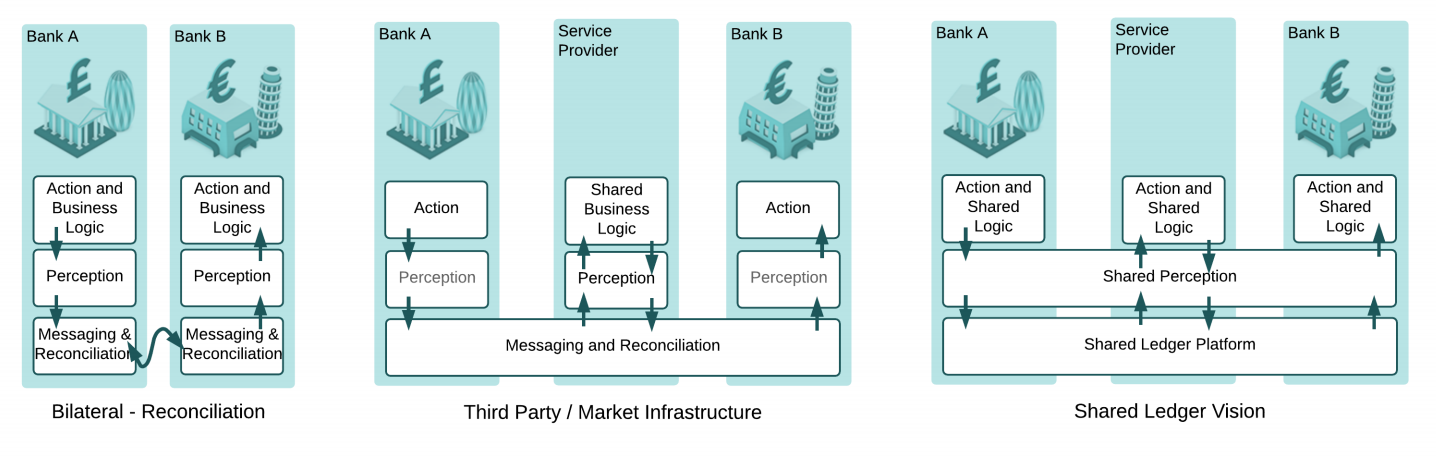
\includegraphics[scale=.5, center]{sharedlogic} 
\caption{En la figura que antecede se muestra la progresión desde un mundo en el que las partes de hechos compartidos registran y gestionan sus propios registros, con las correspondientes discrepancias y duplicaciones (\textit{``Bilateral - Reconciliación"}) o desde un mundo en el que las partes delegan el control y responsabilidad sobre los procesos lógicos a servicios centralizados (\textit{``Terceros / Infraestructura de Mercado"}), a uno en el que estas partes colaboran para mantener un registro compartido, que se garantiza que será consistente entre ellas, utilizando los servicios de proveedores existentes y nuevos, y de proveedores de infraestructura de mercado, siguiendo criterios abiertos y competitivos (\textit{``Visión de un Registro Contable Compartido"}).}
\end{figure}


Creemos que el ahorro derivado de una mayor calidad en los datos, de menores discrepancias y de una más rápida conformidad sobre los detalles entre las empresas será significativo. Por otra parte, la implantación en las empresas de esta arquitectura común definirá una nueva plataforma sobre la cual los proveedores existentes y los nuevos puedan competir para atender a las necesidades de los clientes. Yendo más allá, es posible que esa plataforma también pueda ser utilizada en las propias empresas, en las que el problema de múltiples sistemas que registran datos relativos a las mismas operaciones es también un generador importante de coste y complejidad.

\section{Visión}
A largo plazo es posible imaginar un «registro contable lógico global» con el que interactuarán todos los actores económicos y que permitirá a cualesquiera partes interesadas registrar y gestionar acuerdos entre ellas de forma segura, coherente, fiable, privada y fehaciente. Decimos que es global en el sentido de que todo el mundo ve los mismos datos relevantes para ellos, y lógico en el sentido de que los componentes de la implantación física pueden ser distintos. Como tal, una posible situación final es aquella en la que se haya evolucionado desde sistemas de registro fehacientes y mantenidos dentro de las empresas, a sistemas de registro fehacientes globales compartidos \textit{entre} las empresas. 

\subsection{Principios en la situación final}
Los principios subyacentes a una posible situación final que utilice la tecnología de registro contable distribuido pueden incluir:
\begin{itemize}
	\item Los hechos registrados en el registro contable son considerados por contrato como prueba admisible y legalmente vinculante por todas las partes en caso de disputa.
	\item Los hechos registrados por el registro contable son considerados fehacientes en lugar de «sombras» de datos fehacientes alojados en otro lugar, permitiendo así que las liquidaciones se produzcan directamente en la plataforma.
	\item Una vez todas las partes de un acuerdo hayan manifestado su aprobación, los hechos registrados en el registro contable son finales e inmutables; los errores y reversiones deben ser procesados en una transacción posterior. Las empresas estarán sometidas a la presión de restructurar sus procesos internos para incrementar la precisión y calidad.
	\item Cualquier actor autorizado puede, en principio, conectarse directamente al registro contable y utilizarlo para registrar acuerdos con sus contrapartes. Ningún actor está obligado a tratar con otro pero es posible que veamos un declive de los modelos de mercado «estratificados» o jerárquicos. 
	\item Al promover estándares abiertos y acceso incluyente, tanto los proveedores de servicio ya existentes como los nuevos pueden conectarse y competir para ofrecer servicios diferenciados, promoviendo la competencia y la posibilidad de elegir.
	\item Las únicas partes que deberían tener acceso a los detalles de una transacción financiera son las partes involucradas en dicha transacción y aquéllas que tengan un interés legítimo en conocerlos.
\end{itemize}

No obstante, esta visión incluye la noción de estados transitorios, como los que primero se centrarán en compartir únicamente la lógica de negocio. Esto tiene el objetivo de reconocer la realidad de que los sistemas actuales van a estar con nosotros durante el futuro previsible, lo que requiere vías de coexistencia, integración y migración como parte fundamental de la solución de diseño. Estas fases transitorias pueden resultar también considerablemente valiosas al tratarse en paralelo las implicaciones legales y otras implicaciones no técnicas de la visión a largo plazo.

Es necesario señalar que, con la visión a largo plazo de un registro contable lógico global, se pretende encaminar la dirección, pero que su realización puede ser en forma de una multiplicidad de registros contables. Es posible que adopte la forma de un registro contable por clase de activo, que será autónomo y ligeramente conectado, y que proporcione independencia operativa y funcional entre distintos servicios empresariales. 

Las opciones arquitectónicas y estratégicas que subyacen en esta visión incluyen:
\begin{itemize} 
\item Los registros gestionados por este sistema solamente serán accesibles para los actores que tengan un interés legítimo en los activos y acuerdos que gestionen.
\item El comportamiento de los acuerdos gestionados por el sistema estará descrito en código informático que haga referencia explícitamente a un clausulado prevalente del que obtiene su legitimidad.
\item Se proporcionará soporte para las actualizaciones del código contractual y referencia explícita a los procedimientos de resolución de disputas con el fin de proporcionar certeza en la presencia de contratos fallidos. Esto se debe a que pueden surgir disputas contractuales incluso en un entorno automatizado, como consecuencia tanto de factores humanos como técnicos. 
\item La implantación con éxito de esta visión se conseguirá, mediante una reducción de costes, riesgos y carga regulatoria (incluyendo obligaciones de capital, de liquidez y operativas) y haciendo posibles nuevos procesos y servicios que sean innovadores.
\item Para conseguir ser ampliamente adoptado en la comunidad financiera, partes del sistema deben ser abiertos, y lo serán: código abierto, proceso de desarrollo abierto, estándares abiertos.
\item Aunque esta visión habla en términos de «plataforma» o «sistema», creemos que el diseño será, de hecho, de multinivel, con distintos proveedores compitiendo/colaborando potencialmente para ofrecer distintos elementos. Los lectores no deben suponer que nuestra perspectiva es monolítica integrada verticalmente.
\item Esta visión incluye también la posibilidad de que los niveles superiores de la “pila†puedan contener IP propietario de empresas o grupos concretos.
\item Este sistema funcionará bajo la asunción de un entorno de seguridad desfavorable: es necesario partir de la creciente amenaza del ciberdelito.
\end{itemize}

Se considera que las invenciones fundamentales necesarias para implantar esta visión ya existen e incluyen, sin limitarse a ello, criptografía sólida, redes de comunicaciones globales, estándares para la definición de instrumentos financieros y algoritmos eficaces para asegurar la consistencia a escala global. 

Lo que hace posible hoy en día esta visión es el hecho de que el reciente interés popular en un registro contable distribuido y los sistemas de cadena de bloques han creado un entorno en el que dicha visión puede ser discutida abiertamente, y que se ha constituido una iniciativa común en la que múltiples instituciones financieras pueden actuar juntas. Ello supone una infraestructura de identidad entre los participantes de la red, pero no presupone nada en cuanto a su sofisticación o modo de operar. El compromiso regulador es un elemento clave del proceso de diseño.

A partir de nuestro análisis y evaluación de los requisitos de las plataformas de registro contable distribuido hemos llegado a la conclusión de que ninguna de las plataformas existentes satisface nuestras necesidades.  En esencia, el modelado de amenazas que subyace al diseño de las bases de datos tradicionales distribuidas es inadecuado para nuestro escenario de uso en el que se pretende alcanzar el consenso entre entidades legales entre las que no exista una relación de confianza. Por otro lado, las arquitecturas de sistemas de cadena de bloques existentes resultan inadecuadas para nuestros requisitos de compartición de datos de forma restringida y minuciosa especificada a nivel de acuerdos legales concretos.  Como consecuencia hemos diseñado Corda e iniciado su desarrollo.

\section{Corda}
Corda es una plataforma de registro contable distribuido para el registro y proceso de acuerdos financieros, diseñado para llevar a efecto la visión contenida en este documento.  

La plataforma de Corda sustenta contratos inteligentes, ajustándose a la definición de Clack, Bakshi, Braine.\cite{SCT} Nuestro contrato inteligente es un acuerdo cuya ejecución es \textit{automatizable} mediante código y que trabaja con entrada y control humanos, al tiempo que sus derechos y obligaciones, tal y como se expresan en el clausulado, son legalmente \textit{exigibles}.  El contrato inteligente enlaza la lógica de negocio y los datos de negocio con el clausulado asociado con el fin de garantizar que los acuerdos financieros de la plataforma tengan una base legal firme y sean exigibles, y que el camino a seguir, en el caso de ambigüedad, incertidumbre o disputa, sea claro.

\subsection{Características principales}
Corda se ha especializado para ser utilizada con instituciones financieras reguladas. Se inspira en gran medida en los sistemas de cadena de bloques, pero sin las opciones de diseño que hacen que éstos resulten inadecuados para muchos escenarios financieros. 

Corda proporciona un marco en el que ejecutar contratos inteligentes que cuenta con estas características y actividades clave:
\begin{itemize}
    \item{Registro y gestión de la evolución de los acuerdos financieros y otros datos compartidos entre dos o más partes identificables de una forma basada en las construcciones legales existentes y compatible con la regulación existente y emergente}
    \item{Coordinación del flujo de trabajo entre empresas sin un controlador central.}
    \item{Soporte del consenso entre empresas a nivel de operaciones concretas no a nivel global de sistema.}
    \item{soporte de la inclusión de nodos observadores reguladores y supervisores.}
    \item{Validación de las transacciones únicamente entre las partes de las mismas.}
    \item{Soporte de una diversidad de mecanismos de consenso.}
    \item{Registro enlaces explícitos entre el clausulado humano y el código de los contratos inteligentes.}
    \item{Uso de herramientas estándar de la industria.}
    \item{Limitación del acceso a los datos de un acuerdo a aquellos que cuenten con el derecho explícito o privilegio lógico.}
\end{itemize}
Estas características contribuyen al diseño de una plataforma apropiada para organizaciones de servicios financieros complejas. Hay que señalar que este diseño no utiliza una criptomoneda nativa ni impone un límite global de velocidad a las transacciones.

\subsection{Conceptos}
Empecemos con la idea de un registro contable global: una única fuente fiable. Sin embargo, en nuestro modelo las transacciones y los asientos del registro contable no son visibles globalmente. En los casos en los que las transacciones únicamente involucran solo a un pequeño subgrupo de partes, hacemos lo posible por mantener los datos relevantes únicamente dentro de dicho subgrupo. 

El objeto fundacional de nuestro concepto es un \textit{objeto de estado}, que es un documento digital que registra la existencia, el contenido y el estado actual de un acuerdo entre dos o más partes. Se pretende que sea compartido únicamente entre aquellos que tengan un motivo legítimo para verlo. Para garantizar la consistencia en un sistema compartido, global, en el que no todos los datos sean visibles para todos los participantes, nos basamos en gran medida en hashes criptográficos seguros para identificar a las partes y a los datos. El registro contable se define como un conjunto de objetos de estado inmutables.

Hablamos y pensamos en términos del estado de los acuerdos, y nuestro objetivo es garantizar que todas las partes del acuerdo estén de acuerdo en cuanto al estado del mismo según evoluciona. Podría argumentarse que esta es la esencia del concepto de la cadena de bloques: garantizar que los datos mantenidos por distintos actores sean, y sigan siendo, consistentes al aplicarse operaciones de actualización de dichos datos, y que esto constituye la base sobre la que se construyen las transacciones fiables, desde los simples pagos monetarios hasta las transiciones de contratos inteligentes sofisticados.

\begin{figure}[H]
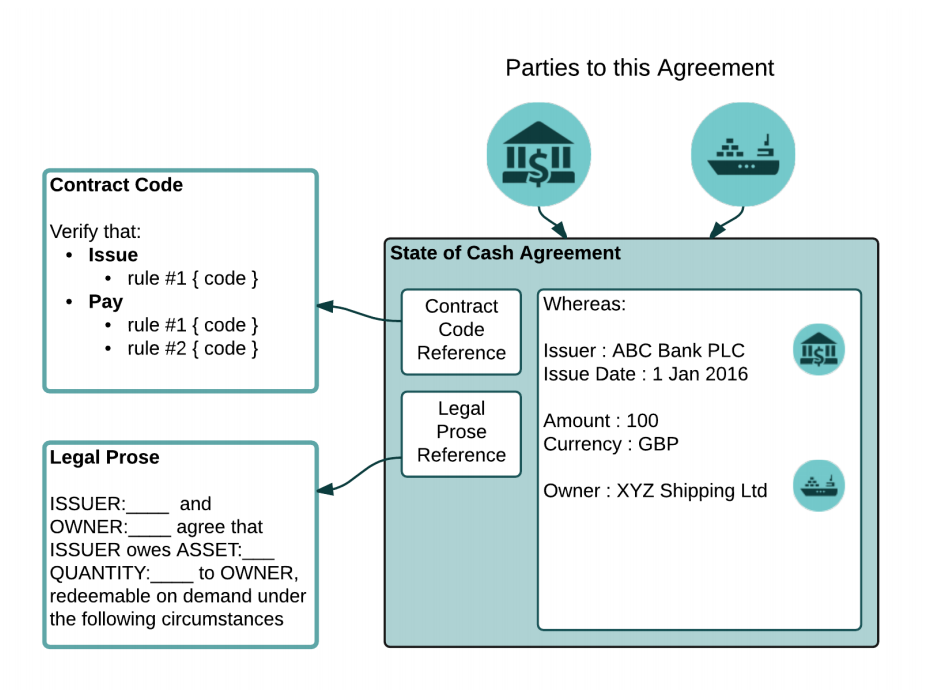
\includegraphics[scale = .4, center]{partiesto}
\caption{En esta figura vemos un objeto de estado que representa una requerimiento de efectivo de \pounds100 contra un banco comercial, propiedad de una compañía de transportes ficticia.  El objeto de estado hace referencia explícitamente, mediante hash, al clausulado que lo regula y al código de contrato que regula sus transiciones.}
\end{figure}

El hecho de que nos centremos en los estados de los acuerdos marca la diferencia respecto a los sistemas en los que los datos sobre los cuales los participantes deben llegar al consenso, son el estado de todo un registro contable o el estado de toda una máquina virtual. Corda proporciona tres herramientas principales para alcanzar el consenso distribuido global:
\begin{itemize}
    \item Lógica de contratos inteligentes para garantizar que las transiciones de estados son válidas con arreglo a reglas acordadas previamente.
    \item Servicios de singularidad y registro de fecha y hora para ordenar las transacciones por tiempo y eliminar conflictos.
    \item Marco de coordinación que simplifica el proceso de escribir protocolos multicapa complejos entre múltiples partes distintas.
    \end{itemize}
    
\subsection{Consenso}
En Corda se aplican las actualizaciones utilizando \textit{transacciones}, lo que consume los objetos de estado existentes y produce nuevos objetos de estado. El consenso tiene dos aspectos:
\begin{enumerate}
\item{Validez de la transacción: las partes pueden confirmar sin ninguna duda que la actualización propuesta de una transacción que define estados de salida es válida verificando que el código de contrato asociado se ejecuta satisfactoriamente y tiene todas las firmas necesarias, y que todas las transacciones a las que hace referencia esta transacción son también válidas.}
\item{Singularidad de la transacción: la partes pueden confirmar sin ninguna duda que la transacción en cuestión es el único consumidor de todos sus estados de entrada, esto es: no existe ninguna otra transacción, sobre la cual se haya alcanzado previamente el consenso (validez y singularidad), que consuma cualquiera de los mismos estados.}
\end{enumerate}

Las partes pueden acordar la validez de una transacción ejecutando independientemente el mismo código de contrato y la misma lógica de validación. En cambio, el consenso sobre la singularidad requiere un observador predeterminado, que en muchos casos tendrá que ser independiente.

\begin{figure}[H]
    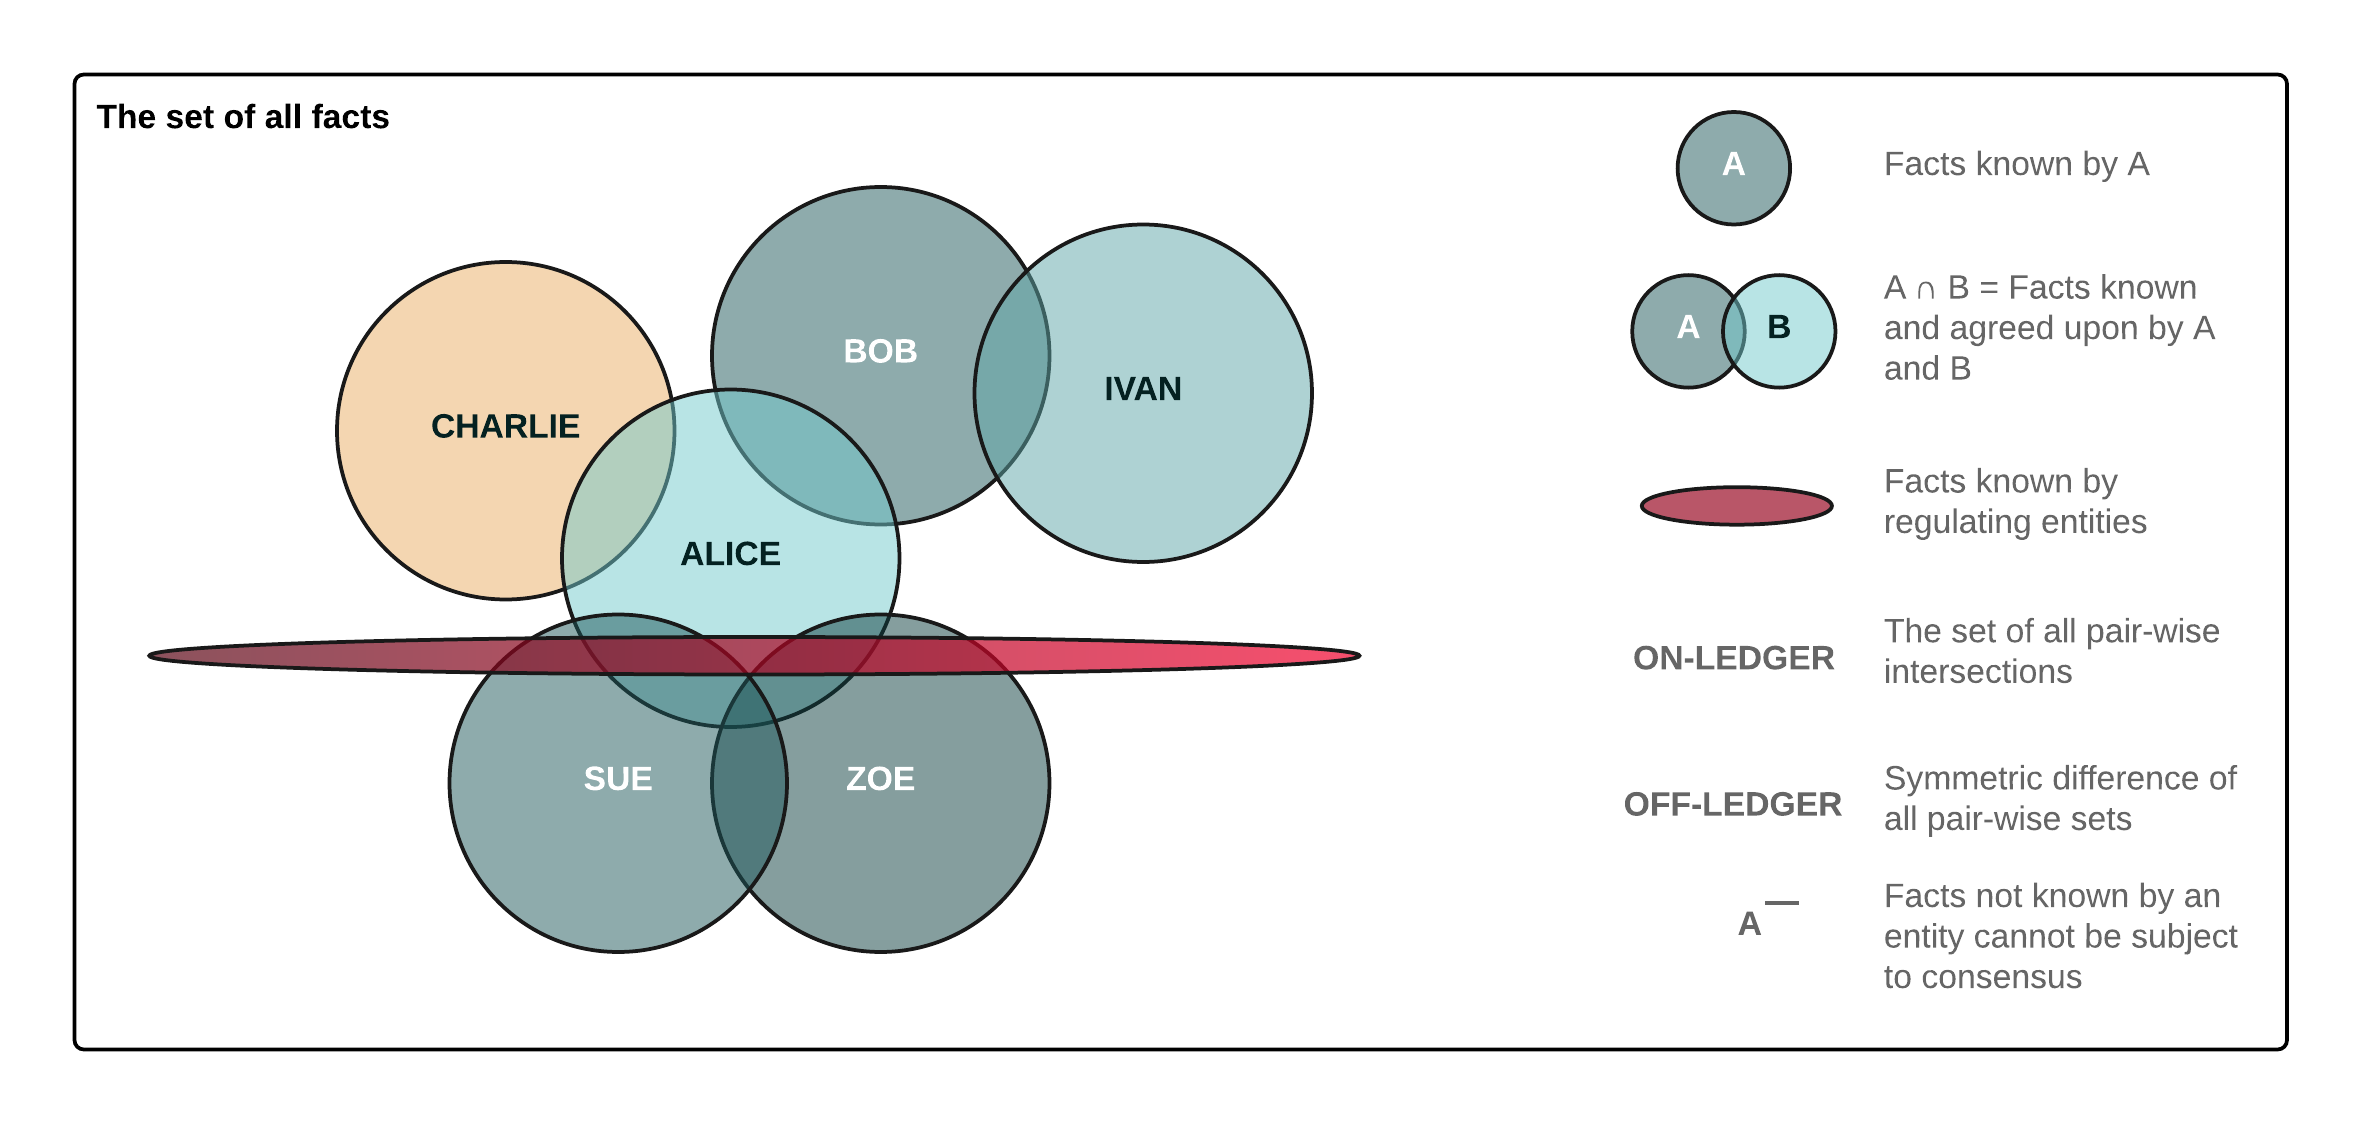
\includegraphics[scale = .5, center]{Consensus}
    \caption{El consenso sobre la validez de una transacción es establecido únicamente por las partes de la transacción en cuestión. De esta forma, los datos son compartidos únicamente por las partes que necesitan verlos. En cambio, el resto de plataformas alcanza en general el consenso a nivel de registro contable. Por ello, cualquier actor de un sistema Corda únicamente ve un subgrupo de los datos globales gestionados por el sistema como un todo. Decimos que un dato está «on-ledger» (en el registro contable) si existe consenso entre, como mínimo, dos actores del sistema respecto a su existencia y detalles, y permitimos la participación de combinaciones arbitrarias de actores en el proceso de consenso para cualquier dato concreto. Los datos que solamente tienen un actor están «off-ledger» (fuera del registro contable).}
\end{figure}

Corda dispone de servicios de singularidad conectables. Su finalidad es mejorar la privacidad, la escalabilidad, compatibilidad con los sistemas legales\cite{EUC} y la agilidad algorítmica. Un único servicio puede estar compuesto por muchos nodos entre los que no existe relación de confianza que se coordinan mediante un algoritmo bizantino de tolerancia de fallos, o puede ser muy simple, como una única máquina. En algunos casos, como cuando cambiar un estado requiere las firmas de todas las partes relevantes, puede no ser necesario en absoluto el servicio de singularidad. 

Es importante señalar que estos servicios de singularidad son necesarios únicamente para certificar si los estados consumidos por una transacción determinada han sido consumidos previamente. No son necesarios para certificar la validez de la transacción misma, que es incumbencia de las partes de la transacción. Esto significa que los servicios de singularidad no son necesarios (y en general no lo serán) para ver todos los contenidos de las transacciones, lo que mejora significativamente la privacidad y escalabilidad del sistema con respecto a otros diseños de registros contables distribuidos y cadenas de bloques.  Esta decisión de diseño representa una elección importante en cuanto a las concesiones que deben realizar las arquitecturas de registros contables, y se analiza en mayor profundidad en un artículo técnico de próxima publicación.

\subsection{Lógica de negocio}
Corda fortalece la lógica de negocio mediante código de contratos inteligentes, construido como una pura función que acepta o rechaza una transacción y que puede estar compuesto de funciones simples reusables. La interpretación de las transacciones que hacen estas funciones toma los estados como entrada y produce estados de salida mediante la aplicación de comandos (contrato inteligente) aceptándose la transacción si las acciones propuestas son válidas. Los contratos definen parte de la lógica comercial del registro contable, y son móviles: los nodos se descargarán y ejecutarán contratos dentro de una sandbox sin revisión alguna en ciertas implementaciones, aunque nos planteamos el uso de código firmado para las implementaciones de Corda en la esfera regulada. 

La máquina virtual que hemos seleccionado para la ejecución y validación del contrato es la Máquina Virtual Java\cite{JVM}, ya que cuenta con numerosísimas bibliotecas y una amplia base de conocimientos, y reutilizar un estándar de la industria facilita que los bancos puedan reutilizar en los contratos el código existente. No obstante, la ampliamos con una sandbox personalizada que es radicalmente más restrictiva que la sandbox normal de la JVM, y refuerza no solo los requisitos de seguridad sino también la ejecución determinista. Al igual que Ethereum\cite{Ethereum}, la elección de estandarizar un bytecode en lugar de un lenguaje permite a los usuarios innovar en el diseño del lenguaje de contratos, o reutilizar lenguajes conocidos, según prefieran. También facilita el uso directo del código de contratos desde aplicaciones internas, una vez se haya revisado el contrato, lo que debería simplificar considerablemente el desarrollo de aplicaciones.

\subsection{Conceptos financieros esenciales}
La arquitectura de Corda está muy influenciada por tres \textit{escenarios de uso arquitectónicamente significativos} que se considera que representan los problemas comunes que es probable que tenga que abordar.  Estos tres escenarios son: efectivo, valores y contratos de derivados. Consideramos los tres casos como ejemplos de acuerdos financieros:
\begin{itemize}
\item Saldo de efectivo (p.ej., «El banco indicado a continuación y yo acordamos que me deben \$1 millón»).
\item Un valor en custodia (p.ej., «El banco custodio indicado a continuación y yo acordamos que soy el titular de 1000 acciones de la sociedad indicada a continuación»).
\item Un acuerdo de derivados bilateral (p.ej., «Los Bancos A y B acuerdan que son partes del siguiente Swap de Tipos de interés (IRS), lo que significa que acuerdan permutar los siguientes flujos de efectivo (compensados) en unas fechas predeterminadas planificadas con una fórmula de liquidación acordada»).
\end{itemize}
Tomando uno de estos ejemplos, el diseño de efectivo de Corda modela directamente la realidad empresarial de que la realidad de «dinero en un banco» no existe realmente, sino solamente un derecho a efectivo que tiene el titular respecto a una institución determinada.\cite{BOE} Así, el contrato de efectivo de Cash es extremadamente simple, pero eficaz: registramos la identidad legal del emisor del efectivo, la moneda, el importe, el titular (y demás información sobre la naturaleza del derecho, con un enlace explícito al \textit{clausulado} que regula el acuerdo, que se prevé que especifique también los procedimientos de resolución en caso de disputa) y lo utilizamos para construir todos los demás conceptos relativos al efectivo (pagos, compensación, etc.)
\begin{figure}[H]
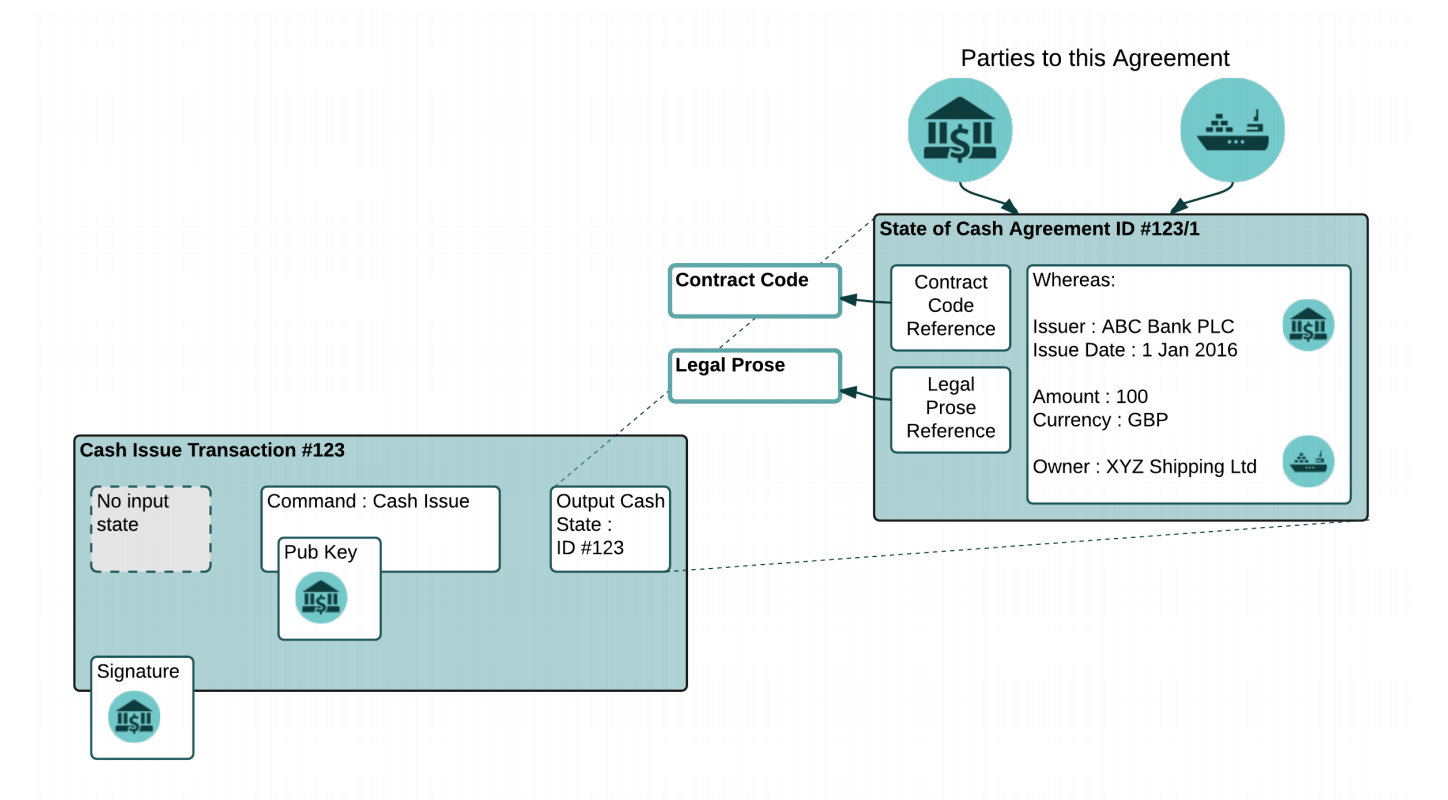
\includegraphics[scale = .4, center]{cash}
\caption{En esta figura vemos una de las transacciones más simples de Corda: una transacción de emisión.  Vemos la creación de un nuevo estado Cash, emitido por un banco comercial a una empresa de transportes ficticia. La transacción de emisión está firmada por el banco emisor.  A partir de este modelo simple pueden construirse transacciones más complicadas, como pagos, contratos de entrega contra pago y obligaciones futuras.}
\end{figure}
\subsection{Resumen del Modelo Corda}
Los conceptos fundamentales de nuestro modelo son:
\begin{itemize}

\item \textit{Objetos de estado}, que representan un acuerdo entre dos o más partes, regulado por \textit{Código de Contrato} en lenguaje máquina. Este código hace referencia a secciones del \textit{Clausulado} en lenguaje humano, que está previsto implantar. \item \textit{Transacciones}, que hacen pasar a los objetos de estado por un ciclo de vida.
\item \textit{Protocolos de Transacción} o \textit{Flujo de Negocio}, que permiten a las partes coordinar acciones sin un controlador central.
\end{itemize}

El determinismo es maximizado y la cantidad de estados requeridos se minimiza restringiendo selectivamente y de forma decisiva el universo de técnicas de programación permisibles.

Es posible concebir la combinación de objetos de estado (datos), Código de Contrato (operaciones permisibles), Protocolos de Transacción (coordinación de la lógica de negocio), todas las API necesarias, pluggins de monedero electrónico (wallet), y componentes de interfaz de usuario, como una aplicación de Registro Contable Compartido, o Aplicación Distribuida de Corda (\textit{``CorDapp"}). Este es el conjunto fundamental de componentes que se espera que un desarrollador de contratos construya en la plataforma. 

%\begin{figure}[H!]
%\includegraphics[scale = .4, center]{image4}
%\caption{Planteamiento actual de las aplicaciones en el ecosistema organizado con Corda.}
%\label{fig:figure4}
%\end{figure}

%\begin{figure}[H!]
%\includegraphics[scale = .25, center]{image5}
%\caption{Otra representación visual de cómo Corda interactuará con el ecosistema financiero.}
%\label{fig:figure5}
%\end{figure}

\section{Comparación con otras plataformas}
Corda fue creado a partir de una colaboración exhaustiva con profesionales del sector financiero y está diseñado teniendo en mente sus requisitos. Sin embargo, su diseño está también inspirado en trabajos anteriores, como por ejemplo el presentado en los escritos de Todd Boyle e Ian Grigg sobre la contabilidad triangular \cite{Triple}, y aspectos de las plataformas de registro contable distribuido existentes, tales como Bitcoin\cite{Bitcoin} y Ethereum. Por eso quizá sea más fácil para los que no conocen Corda entenderlo en los términos de esas plataformas. 

\subsection{Comparación con Bitcoin}
Corda tiene unas semejanzas significativas con Bitcoin: 
\begin{itemize}
\item{La idea de estados inmutables que son consumidos y creados por transacciones es la misma.}
\item{Transacciones con múltiples inputs y outputs. Por ello, Bitcoin a menudo hace referencia al registro contable como el conjunto de output de transacciones no utilizadas (conjunto UTXO).}
\item{Un contrato es una función pura; los contratos no tienen almacenamiento ni capacidad de interaccionar con otros elementos. Dadas las mismas transacciones, la función «verify» (verificar) de un contrato siempre produce exactamente el mismo resultado.}
\end{itemize}

Sin embargo, una transacción Bitcoin tiene un formato de datos único, rígido, y puede alojar muy pocos datos, aparte de cantidades de bitcoin y las normas de gasto asociadas (script). Se sabe que algunos han intentado resolver esta limitación integrando los datos en lugares semiestandarizados en el código del contrato, de forma que se puedan extraer los datos por concordancia de patrones, pero este enfoque resulta insuficiente. En cambio, nuestros estados pueden incluir datos de tipo arbitrario. Adicionalmente, nuestras transacciones no solamente llaman a los contratos de input, sino también a los contratos de los outputs. La aceptación de una transacción Bitcoin está controlada únicamente por el código del contrato en los estados de input consumidos. Utilizamos el término «contrato» para hacer referencia a un paquete de lógica de negocio que puede gestionar diversas tareas, además de la verificación de la transacción. Por ejemplo, actualmente nuestros contratos incluyen también código para la creación de transacciones válidas (lo que a menudo es denominado «código wallet» en Bitcoin).


A un script de Bitcoin solamente se le puede dar como entrada un conjunto fijo de matrices de bytes. Esto significa que un contrato no tiene forma de examinar la estructura de toda la transacción, lo que limita severamente lo que pueden hacer los contratos. Nuestros contratos son Turing completos y pueden estar escritos en cualquier lenguaje de programación habitual destinado a la JVM.	
Corda permite especificar límites de tiempo arbitrariamente precisos en las transacciones (que deben ser certificados por un registrador de fecha y hora fiable) en lugar de basarse en la hora en la que se extrae la información de un bloque.  Esto es importante ya que muchos de los tipos de contratos que contemplamos sustentar requieren precisión en cuanto al tiempo y porque nuestras implantaciones primarias de consenso utilizan algoritmos de resolución de conflictos sin bloques. Es necesario señalar que Corda no utiliza «Proof of Work» ni el concepto de «minería».

\subsection{Comparación con Ethereum}
Como en el caso de Ethereum, el código se ejecuta en una máquina virtual relativamente potente y puede contener lógica compleja. Para la programación de los contratos pueden utilizarse lenguajes de programación no basados en ensamblaje.  Ambos están destinados al modelado de muchos tipos distintos de contratos financieros.

Sin embargo, el término «contrato» en Ethereum hace referencia a la instanciación de un programa que es replicada y mantenida en todos los nodos participantes. Esta instanciación es muy similar a un objeto de un programa Orientado a Objeto: puede recibir y enviar mensajes, actualizar el almacenamiento local, etc. En cambio, nuestra implantación de los contratos inteligentes en código hace referencia a un conjunto de funciones, de las cuales solamente una participa en el mantenimiento de la sincronización del sistema (la función \textit{verify}). Esta función es pura y sin estado (esto es, puede no interactuar con ninguna otra parte del sistema mientras se ejecuta).	Como los contratos no tienen ningún tipo de almacenamiento mutable, no existe la noción de «mensaje». Ethereum también afirma ser una plataforma no solo para lógica financiera, sino literalmente cualquier tipo de aplicación. Nuestra plataforma considera que las aplicaciones no financieras quedan fuera de nuestro ámbito, al menos inicialmente.

%\section{Ejemplo práctico: Efectivo}
%Un objeto de estado (en la imagen ) representa un acuerdo compartido entre las partes.

%Los estados contienen datos arbitrarios, pero siempre contienen, como mínimo, una referencia al hash de un código de contrato, que es un programa expresado en determinado bytecode que se ejecuta en una sandbox dentro de una máquina virtual, y una referencia al hash de un documento con el clausulado, que proporciona el contexto legal en un formato reconocible por una autoridad judicial u otro sistema de resolución de disputas. \textit{Código de contrato} (o simplemente “Contratos” en el resto de este documento) son elementos de lógica de negocio compartida globalmente. Los contratos siempre definen una función «verify», que es una función pura que puede determinar si la transición del Estado es válida, con independencia de qué parte llama a la función. La función «verify» no comprueba que una transacción sea en el interés de ninguna de las partes, solamente que se respeten sus restricciones, y los propios nodos deben cumplir por separado el requisito de que la transacción sea en su propio interés. Esto se analiza más adelante.

%En esta figura vemos un \textit{objeto de estado efectivo} estilizado, que representa la titularidad de 100 USD. El objeto hace referencia al contrato que lo regula y al clausulado asociado. Como es un contrato de efectivo, el documento con el clausulado especificará los términos y condiciones correspondientes a una responsabilidad por efectivo emitida por una de las partes a la otra: ¿bajo qué circunstancias puede ser redimido el objeto de efectivo?, ¿a cambio de un saldo en una cuenta bancaria tradicional o a cambio de una transferencia a cualquier otro sitio?, ¿Cómo se resolverán las disputas? Etcétera. Además, el clausulado que especifica esos derechos, obligaciones y condiciones asociadas al contrato que las partes acuerdan será automatizado mediante código. Delegaremos explícitamente del dominio del clausulado al dómino código.

%Adicionalmente, y crucialmente, el clausulado tendrá también varios elementos de información no especificada: quién es el emisor y cuál es la moneda. El objeto de estado contiene estos campos (vemos que aquí el emisor es Barclays Bank PLC y la moneda es USD). La combinación del clausulado, el código de contrato y los parámetros capturados en el objeto estado, más las firmas digitales pertinentes definen conjuntamente el acuerdo entre las partes.

%A continuación describimos cómo una instancia de un objeto de estado, como el que acabamos de ver, puede hacerse evolucionar y ser procesado y transmitido entre las partes utilizando el resto de los componentes de la arquitectura Corda.

%Nota: A muy alto nivel, este diseño es análogo al «modelo UTXO» como el de Bitcoin, pero tiene también algunas diferencias significativas. La elección de un modelo tipo UTXO en lugar de un modelo cuenta/saldo como el utilizado en Ethereum es deliberada y consciente, y es esencial para las características de escalabilidad y privacidad de la plataforma.

\section{Hoja de ruta}
Para llegar a este diseño, primero hemos simulado y creado el prototipo de los componentes de Corda en código para validar aspectos del concepto. Esta es la lista de algunas extensiones al modelo Corda, aunque no de todas, que se espera lanzar a corto-medio plazo.
\begin{itemize}	
\item Descomposición de las transacciones y mejoras en la singularidad: Incorporación de mecanismos para oscurecer selectivamente porciones de transacciones, incluyendo el ocultamiento de los servicios de singularidad.
\item Sandbox de verificación del contrato: Inclusión explícita en listas blancas durante el tiempo de enlazado de un conjunto agresivamente mínimo de bibliotecas de Java.
\item Un monedero basado en plug-in para inferencia de la posición.
\item Oráculos de cálculo o pasarelas a lógica de negocio propietaria (u otra) (p.ej. Contrapartes Centrales o agentes evaluadores) que puedan ser verificados en el registro contable por los participantes.
\item	Utilización del modelo Corda para gestionar la identidad de los usuarios.
\item Interoperabilidad e integración de los datos, específicamente con respecto al FpML ISO20022, soporte de otros formatos de datos e integración/interoperabilidad con otras plataformas.
\item	Construcción de aplicaciones para datos de referencia.
\item	Mejoras en privacidad utilizando tecnologías como la asignación aleatoria de direcciones, pruebas de conocimiento cero, esquemas de reemisión de activos.
\item	Contratos de referencia para más instrumentos financieros.
\item Soporte nativo de lógica de negocio a nivel de cartera, como por ejemplo agregaciones de objetos de estado.
\end{itemize}
\section{Conclusión}
A diferencia de la mayor parte de registros contables distribuidos y plataformas de cadena de bloques, Corda se construyó con el objetivo explícito de registrar y exigir el cumplimiento acuerdos comerciales entre instituciones financieras registradas; no se pretende que sea una solución general para todos los problemas. Como tal, presenta un planteamiento único de distribución de datos y una semántica de aplicaciones, al tiempo que mantiene las características de los registros contables distribuidos que atrajeron en primer lugar la atención de las instituciones respecto a proyectos tales como R3, esto es, la ejecución fiable de los acuerdos financieros de forma automatizable y exigible.
\bibliographystyle{unsrt}
\bibliography{Ref}

\end{document}
